\chapter{Synchronisation}

\section{Signale}
\begin{description}
	\item[Synchronisation (hier)] dafür sorgen, dass gewisse Abläufe ausgeschlossen sind. Auch: Koordination.
	\item[Signal (auch: Handshake, Meldung, engl. Notification)] Hinweis an einen anderen Thread, dass er weitermachen kann.
\end{description}
Analogie:
\begin{itemize}
	\item Startschuss beim Wettlauf
	\item Staffel beim Staffellauf
	\item Anschlusszug muss warten
	\item Becher vor Kaffeezulauf
\end{itemize}
Ein Signal kann durch eine Sperre implementiert werden:
\begin{itemize}
	\item signalisieren (auch: melden) = freigeben
	\item warten = belegen
\end{itemize}
Das Signal soll garantieren, dass eine gewisse Reihenfolge eingehalten wird.
\begin{lstlisting}
P1:
	S1;
	freigeben(l);
P2:
	belegen(l);
	S2;


           S1
P1 -----|------|--|-----------
P2 -----|----------|--|------|
           warten        S2
\end{lstlisting}
l muss freigegeben worden sein, bevor es wieder belegt werden kann, also findet $S_1$ vor $S_2$ statt. Durch die Verwendung von Signalen schränkt man die Menge der Abläufe ein. Nachteil: \emph{weniger Parallelität}.\\
\\
\textbf{Extremfall:} nur noch eine Reihenfolge möglich; der Ablauf wird seriell. Abgesehen vom Koordinationsaufwand zu einem seriellen Programm dann gleichwertig.

\section[Beispiel: Erzeuger/Verbraucher (1)]{Beispiel: Erzeuger/Verbraucher-Problem, 1. Version}
Erzeuger und Verbraucher sind Threads. Der Erzeuger erzeugt Datenblöcke. Der Verbraucher holt die Datenblöcke ab und verarbeitet sie. Die erzeugten aber noch nicht verbrauchten Datenblöcke werden in einem Puffer (:= Warteschlange) zwischengespeichert.

\subsection*{1. Version}
\begin{tabular}{l r}
Erzeuger & 1\\
Verbraucher & 1\\
Puffergröße & 1
\end{tabular}\\
\\
Thread \emph{erz}:
\begin{lstlisting}
Wiederhole:
	herstellen(datenblock);
	einreihen(puffer, datenblock);
\end{lstlisting}
Thread \emph{verb}:
\begin{lstlisting}
Wiederhole:
	abholen(puffer, datenblock);
	verarbeiten(datenblock);
\end{lstlisting}

Prozeduren:
\begin{lstlisting}
	einreihen(puffer, datenblock):
1		belegen(leer);
2		kopieren(datenblock, puffer); // kopiert Datenblock in Puffer
3		freigeben(voll);

	abholen(puffer, datenblock):
4		belegen(voll);
5		kopieren(puffer, datenblock); // kopiert Puffer in Datenblock
6		freigeben(leer);
\end{lstlisting}

Hauptprogramm:
\begin{lstlisting}
	Sperre voll anlegen; // als belegt
	Sperre leer anlegen; // als belegt
	Threads erz und verb anlegen und laufen lassen;
0	freigeben(leer);
\end{lstlisting}

\subsubsection*{Kausalitätsgraph}
\begin{figure}[H]
	\begin{center}
		\includegraphics[width=.5\textwidth]{res/SynchronisationKausalitätsgraph}
		\label{pic:synkaus}
	\end{center}
\end{figure} 
$\longrightarrow$: Programmreihenfolge; $\dashrightarrow$: Reihenfolge erzwungen durch Signal.

\subsubsection*{Petri-Netz}
\begin{figure}[H]
	\begin{center}
		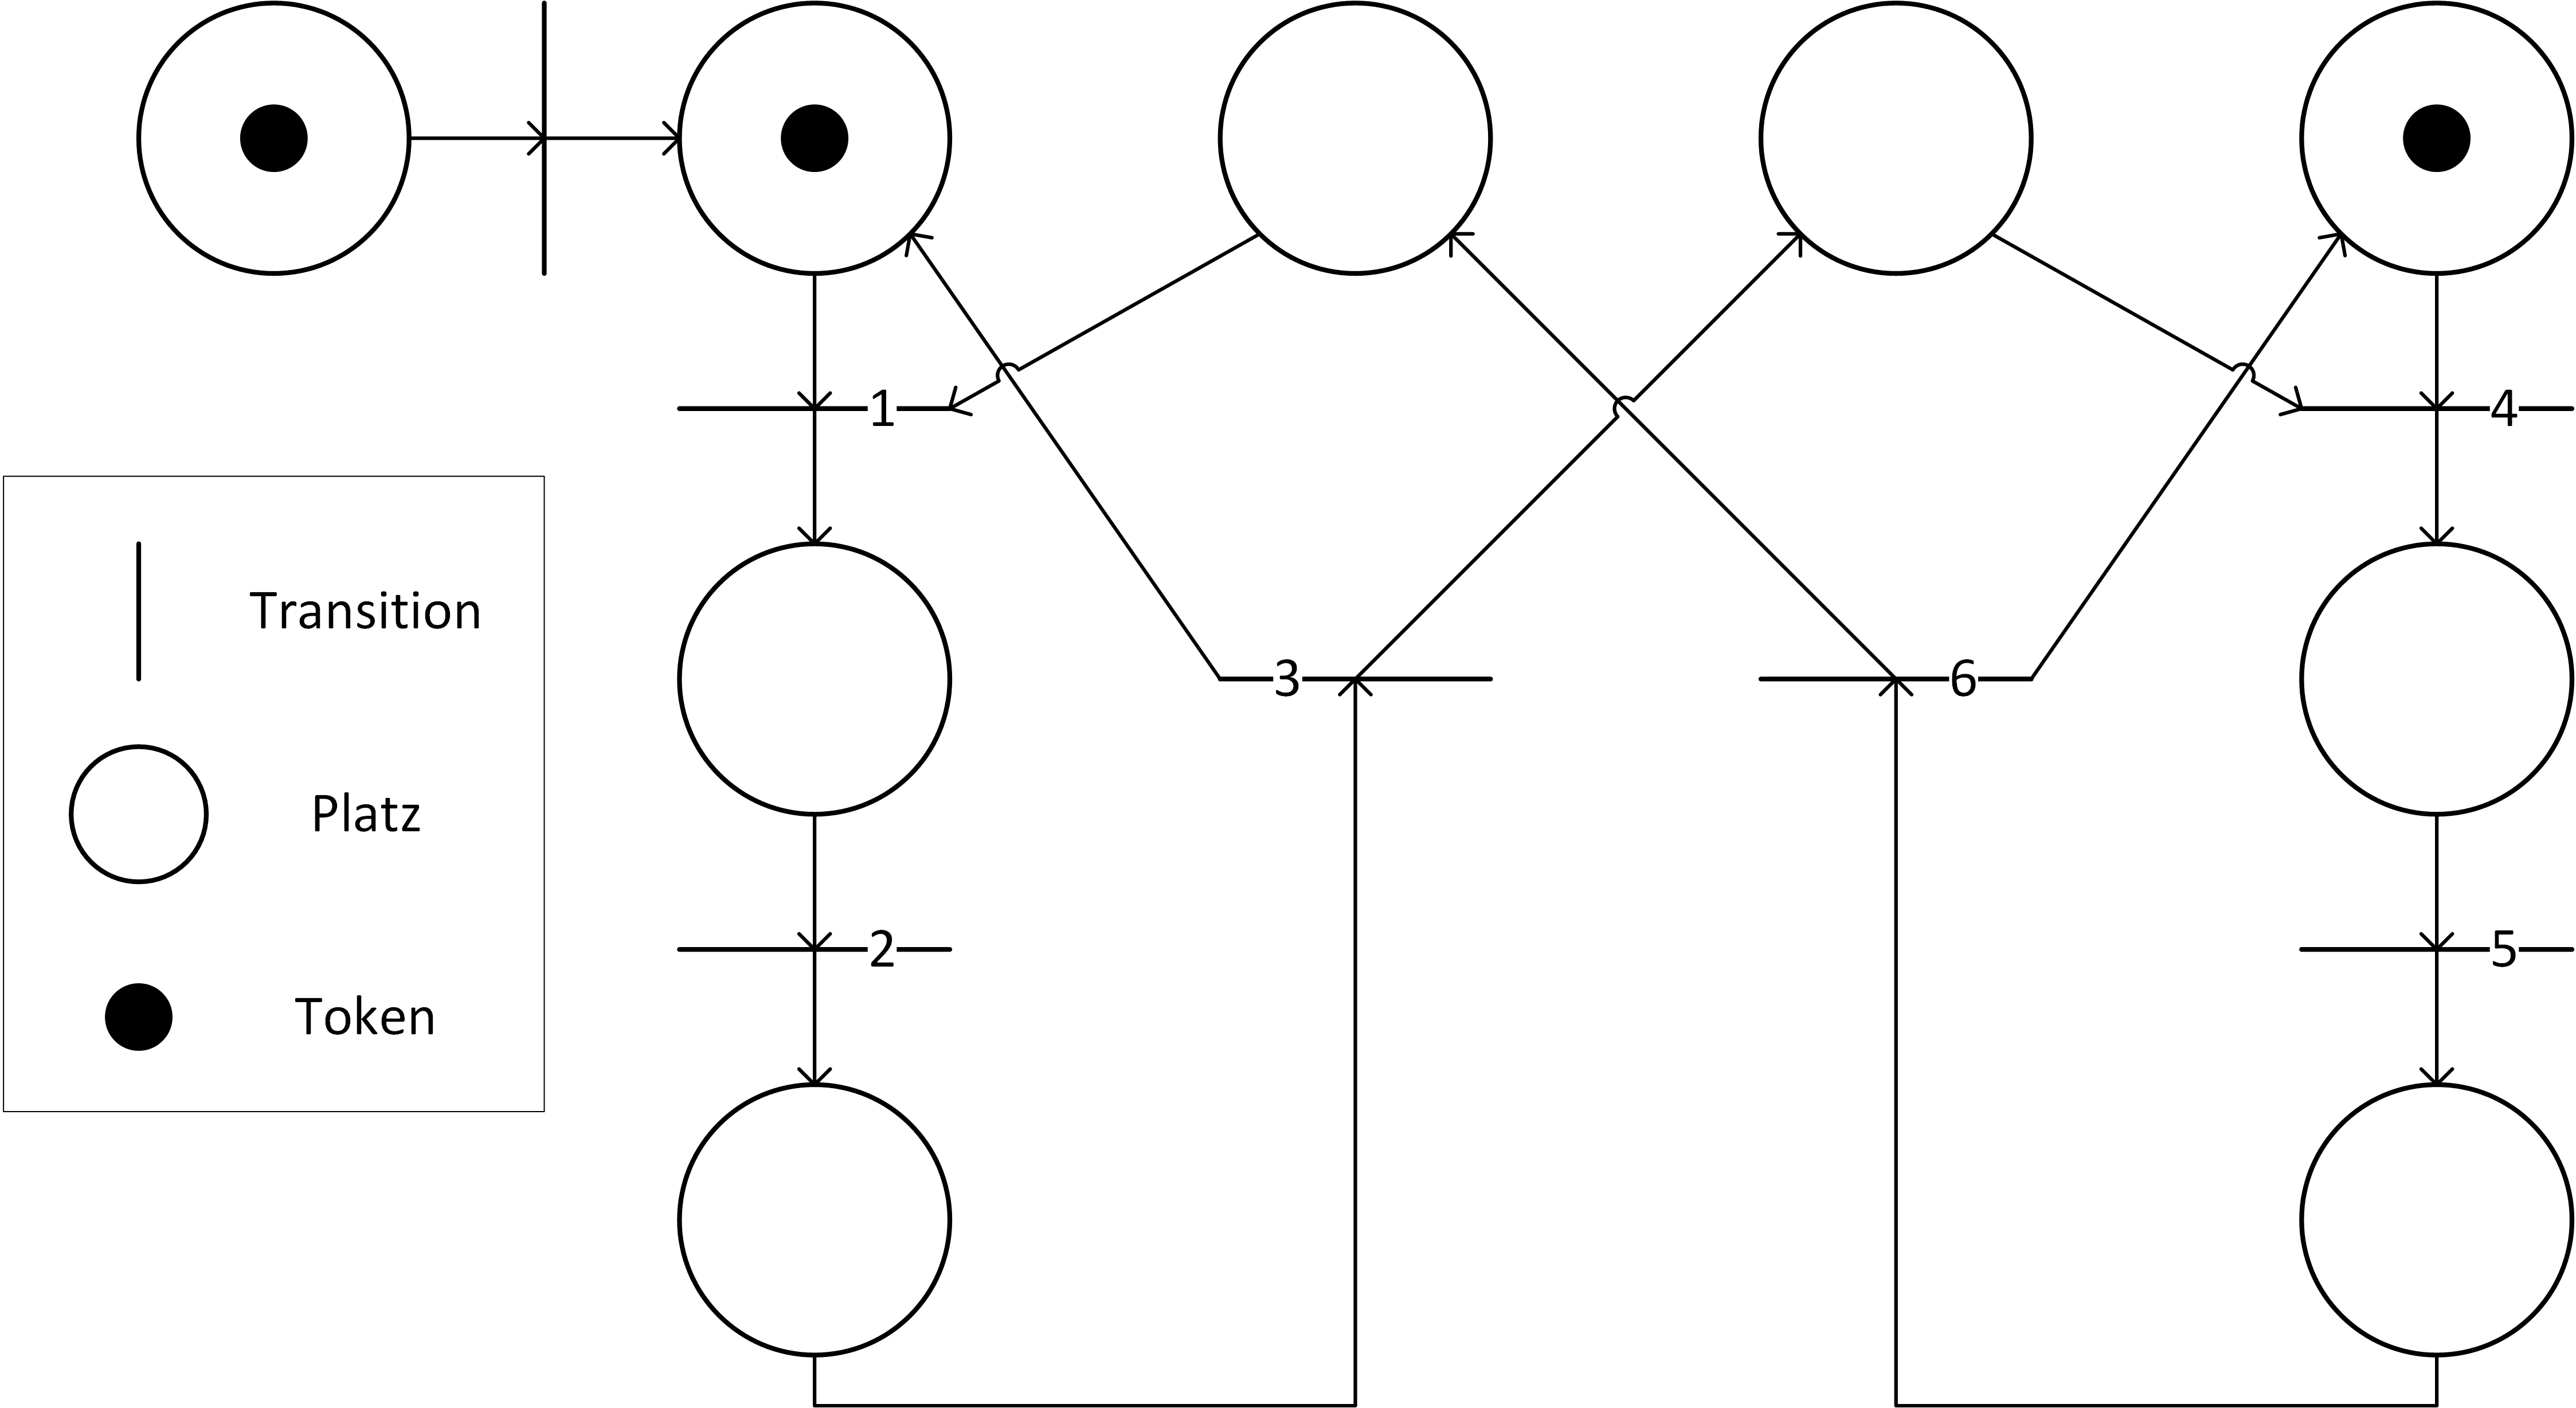
\includegraphics[width=\textwidth]{res/PetriNetz}
		\label{pic:synpetri}
	\end{center}
\end{figure} 
Bipartiter Graph: Zwei Sorten von Knoten; Pfeile nur zwischen verschiedenen Knotensorten.

\subsubsection*{Elementare Ereignis-Struktur}
Durch Abrollen des Kausalitätsgraphen:
\begin{figure}[H]
	\begin{center}
		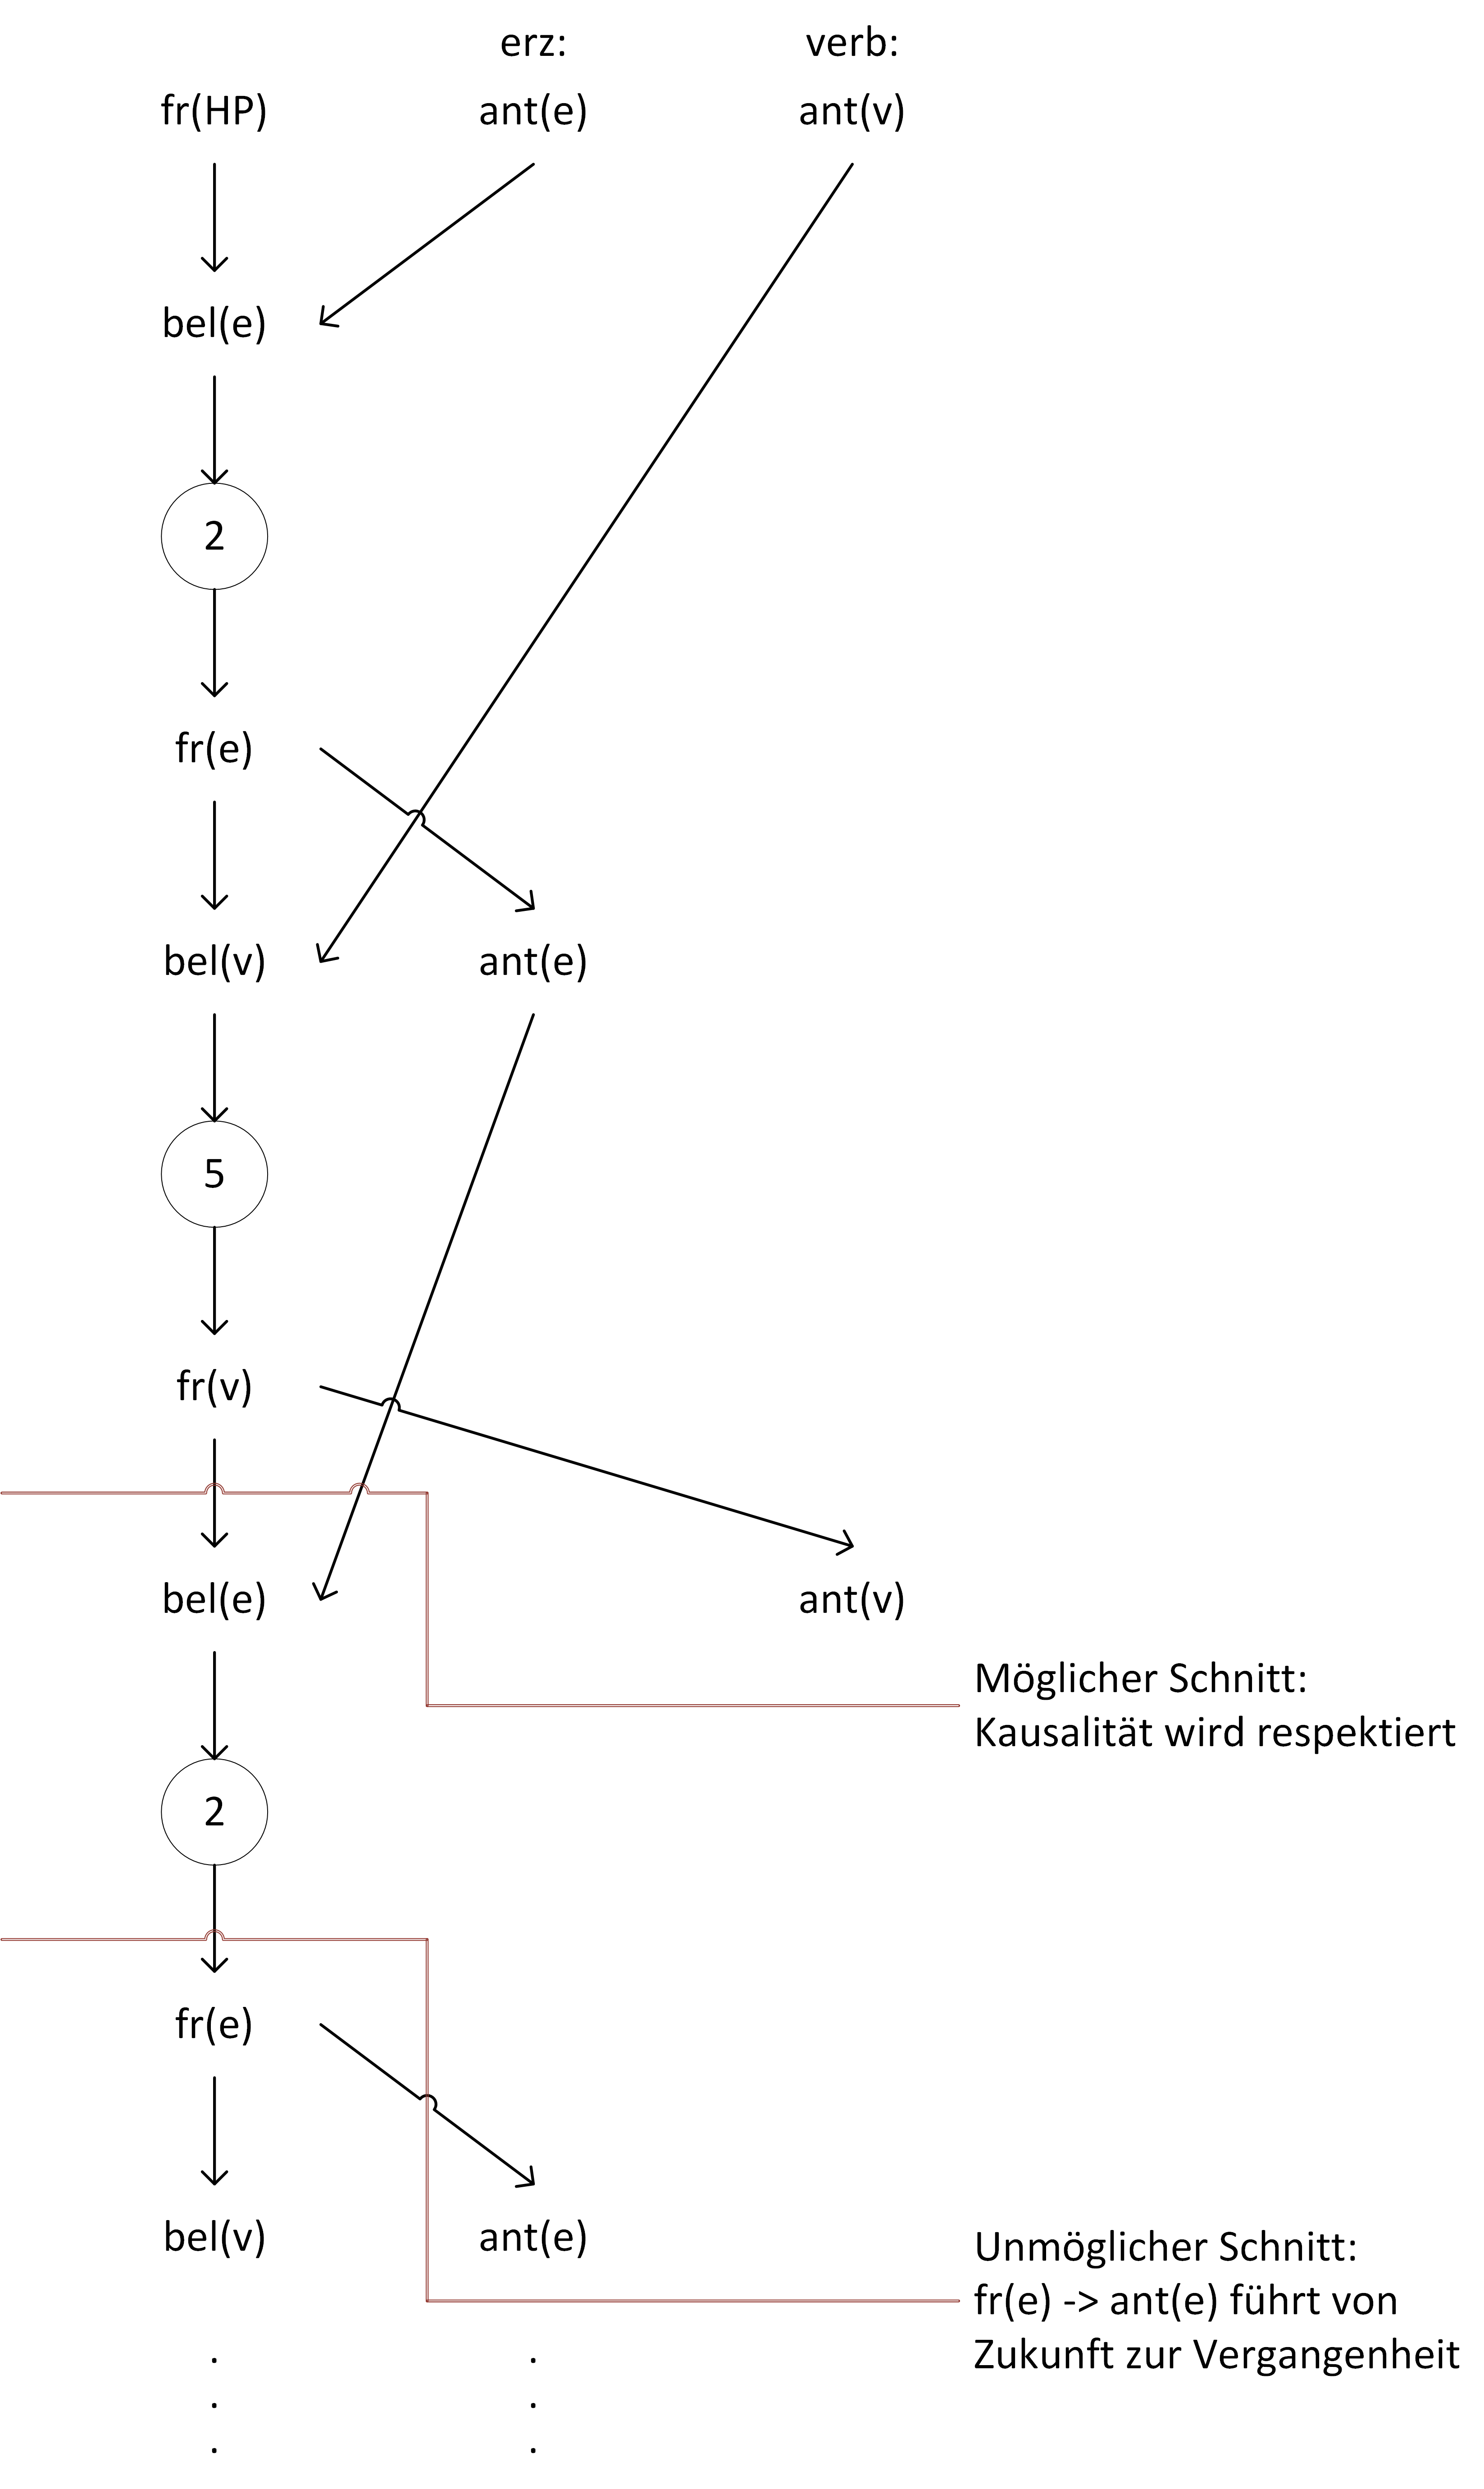
\includegraphics[width=.7\textwidth]{res/ElementareEreignisstruktur}
		\label{pic:synelem}
	\end{center}
\end{figure} 

\subsubsection*{Signaldiagramme}
\begin{figure}[H]
	\begin{center}
		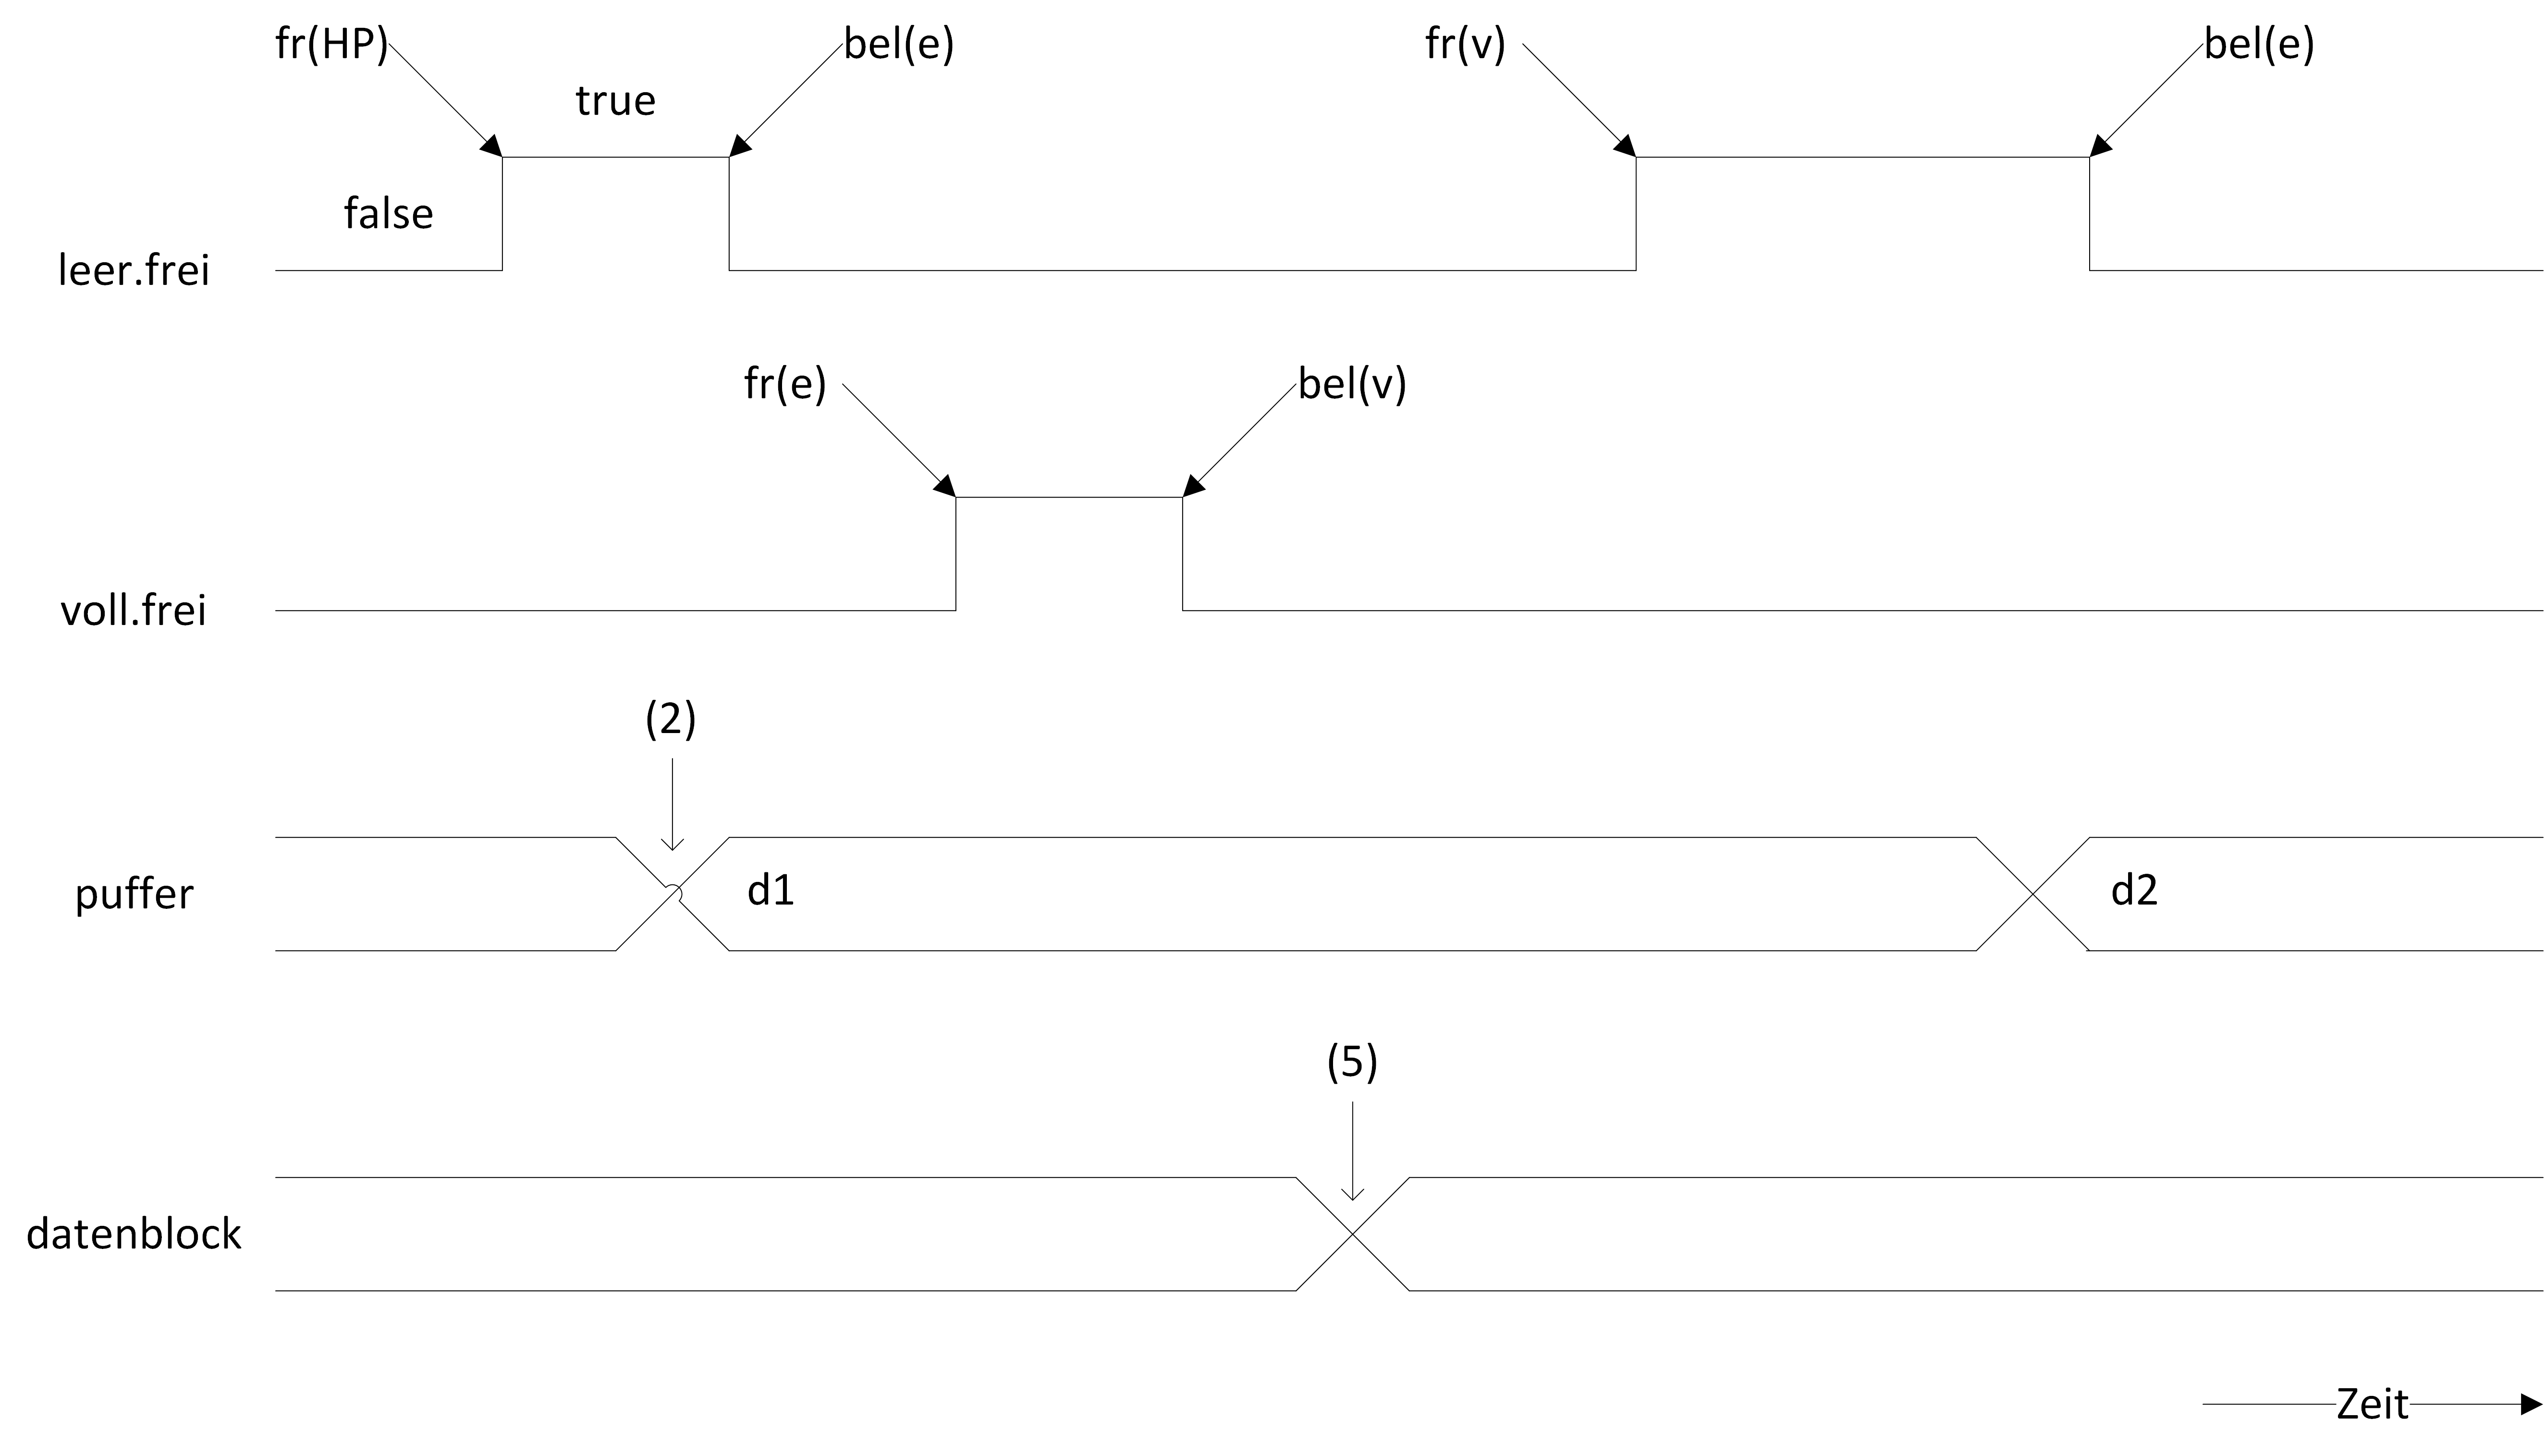
\includegraphics[width=\textwidth]{res/SignalDiagramme}
		\label{pic:synsignal}
	\end{center}
\end{figure} 
\begin{itemize}
	\item (2) und (5) werden als kritische Bereiche behandelt
	\item (2) und (5) werden nur abwechselnd ausgeführt
\end{itemize}
zu 1: Gegenseitiger Ausschluss gilt: $\neg$leer.frei $\lor$ voll.frei ist invariant.\\
zu 2: Folgt aus Programmierreihenfolge und 1.

\section{Semaphore}
\begin{description}
	\item[Semaphor] Datenstruktur mit Zustand l.frei $\in \mathbb{N}_0$ und Operationen "`belegen"' und "`freigeben"'.
	\item[belegen(l)] Wartet bis l.frei > 0 und setzt dann l.frei auf l.frei - 1.
	\item[freigeben(l)] Setzt l.frei auf l.frei + 1
\end{description}
Sperre ist Spezialfall mit l.frei $\in \{0, 1\}$.\\
Zweck: l.frei verschiedene Kopien eines Betriebsmittels werden verwaltet.\\
Zusammenhang zu Klammerausdrücken:\\
"`("' bedeutet "`freigeben(l)"'\\
"`)"' bedeutet "`belegen(l)"'\\
l.frei = Anzahl der noch offenen Klammern\\
\\
Beispiel:
\begin{lstlisting}
                  ( ( ) ( ) )
l.frei 2_|           _   _
       1_|         _| |_| |_
       0_|________|         |_______

\end{lstlisting}
\section[Beispiel: Erzeuger/Verbraucher (2)]{Beispiel: Erzeuger/Verbraucher-Problem, 2. Version}

\subsection*{2. Version}
\begin{tabular}{l r}
	Erzeuger & 1\\
	Verbraucher & 1\\
	Puffergröße & N (mit $N > 0$ beliebig)
\end{tabular}\\
\\
Threads erz und verb wie in Version 1.\\
\\
Prozeduren:
\begin{lstlisting}
	einreihen(puffer, datenblock):
1		belegen(nichtvoll); // I' gilt nun wieder
2		stock(puffer, datenblock); // Anfuegen des Datenblocks an Puffer hinten
3		freigeben(nichtleer); // I gilt
	
	abholen(puffer, datenblock):
4		belegen(nichtleer); // I' gilt
5		datenblock := top(puffer); // Liefert vordersten Datenblock des Puffers
6		pop(puffer);
7		freigeben(nichtvoll); // I gilt

	main():
		Leeren puffer anlegen;
		Semaphore nichtvoll und nichtleer erzeugen mit nichtvoll.frei = 0 und nichtleer.frei = 0;
		Threads erg und verb anlegen und laufen lassen;
		freigeben^N(nichtvoll); // nichtvoll wird N-mal freigegeben
		// I gilt
\end{lstlisting}

Invariante I: $ 0 \leq \text{ nichtvoll.frei } \leq N \land \text{ nichtleer.frei } + \text{ nichtvoll.frei } \leq N $\\
Invariante I': $ 0 \leq \text{ nichtvoll.frei } \leq N \land \text{ nichtleer.frei } + \text{ nichtvoll.frei } \leq N - 1 $\\
Invariante I'': $ 0 \leq \text{ nichtvoll.frei } \leq N \land \text{ nichtleer.frei } + \text{ nichtvoll.frei } \leq N - 2 $\\
I'' gilt, wenn beide Threads belegen, aber noch nicht freigeben aufgerufen haben.

\section{Bedingte kritische Bereiche}
Ein kritischer Bereich soll nur betreten werden, wenn eine gewisse Bedingung B an die gemeinsame Variable gilt. Wie implementiert man das?
\begin{enumerate}
	\item B vor dem Betreten des kritischen Bereichs überprüfen.\\Problem: B kann beim Betreten des kritischen Bereiches bereits wieder verletzt sein.
	\item B im kritischen Bereich überprüfen.\\Problem: Solange B nicht gilt, soll der Thread warten. Weil er sich im kritischen Bereich befindet, können andere Threads die gemeinsame Variable nicht ändern und damit den Wert von B.
\end{enumerate}
Mit kritischen Bereichen kann man das Problem nicht lösen. Abhilfe: neues Konstrukt.

\section[Beispiel: Erzeuger/Verbraucher (3)]{Beispiel: Erzeuger/Verbraucher-Problem, 3. Version}

\subsection*{3. Version}
\begin{tabular}{l r}
	Erzeuger & n\\
	Verbraucher & m\\
	Puffergröße & N (mit $N > 0$ beliebig)
\end{tabular}\\
\\

\section{Wiederbetretbare Sperren}

\section{Leser/Schreiber-Problem}